%\documentclass[a4paper,11pt]{article}%JHEP%
%\pdfoutput=1 % if your are submitting a pdflatex (i.e. if you have
             % images in pdf, png or jpg format)%JHEP%

%\usepackage{jheppub} % for details on the use of the package, please
                     % see the JHEP-author-manual%JHEP%

\documentclass[aps,prd,nofootinbib,preprint]{revtex4}

\usepackage[T1]{fontenc} % if needed
\usepackage{amsmath}
\usepackage{leftidx}
\usepackage{multirow}
\usepackage{enumerate}
%\usepackage{textcomp}

%\usepackage{underscore}
\usepackage[utf8]{inputenc}
\usepackage[english]{babel}

\usepackage[nottoc]{tocbibind}

\usepackage{hyperref}
%\usepackage{ulem}
\usepackage{color}
\usepackage{graphicx}
\usepackage{multirow}
\usepackage{amsmath,amssymb,amsthm,amsxtra,overpic,bbm,bm,float
,epsfig}



%JHEP%
%\title{\boldmath  Flavour Symmetry Embedded - GLoBES (FaSE-GLoBES)}


%JHEP%
%\author[a]{Jian Tang,}
%\author[a]{Tse-Chun Wang}
%\affiliation[a]{School of Physics, Sun Yat-Sen University, Guangzhou 510275, China}
%\emailAdd{tangjian5@mail.sysu.edu.cn}
%\emailAdd{wangzejun@mail.sysu.edu.cn}
%\abstract{Abstract...}


%\fontsize{3}{5}\selectfont
\begin{document} 
%\title{The user manual: FlAvour Symmetry with the GLoBES library}
%\title{FlAvour Symmetry with the GLoBES library}
\title{\Large The user manual: Flavour Symmetry Embedded - GLoBES (FaSE-GLoBES)} %JHEP%
%\maketitle %JHEP%
%\flushbottom %JHEP%
\author{Jian Tang$^1$\footnote{tangjian5@mail.sysu.edu.cn}}
\author{Tse-Chun Wang$^1$\footnote{wangzejun@mail.sysu.edu.cn}}
\affiliation{$^1$School of Physics, Sun Yat-Sen University, Guangzhou 510275, China}

%\begin{abstract}
%\textbf{Keywords: Neutrino Oscillations, Leptonic Flavour Symmetry}  
%\end{abstract}

\maketitle

\section{Introduction}\label{sec:intro}

The discovery of neutrino oscillations points out the fact that neutrinos have mass, and provides evidence beyond the Standard Model (BSM). This phenomenon is successfully described by a theoretical framework with the help of three neutrino mixing angles ($\theta_{12}$, $\theta_{13}$, $\theta_{23}$), two mass-square splittings ($\Delta m_{21}^2$, $\Delta m_{31}^2$), and one Dirac CP phase ($\delta$) \cite{Pontecorvo:1967fh,Maki:1962mu,Pontecorvo:1957qd,Esteban:2018azc}. Thanks to the great efforts in the past two decades, we almost have a complete understanding of such a neutrino oscillation framework. More data in the neutrino oscillation experiments is needed to determine the sign of $\Delta m_{31}^2$, to measure the value of $\sin\theta_{23}$, to discover the potential CP violation in the leptonic sector and even to constrain the size of $\delta$ \cite{Esteban:2018azc}. For these purposes, the on-going long baseline experiments (LBLs), such as the NuMI Off-axis $\nu_e$ Appearance experiment (NO$\nu$A)~\cite{Ayres:2007tu} and the Tokai-to-Kamioka experiment (T2K)~\cite{Abe:2011ks}, can answer these questions with the statistical significance $\gtrsim 3\sigma$ in most of the parameter space. Based on the analysis with their data, the normal mass ordering ($\Delta m_{31}^2>0$), the higher $\theta_{23}$ octant ($\theta_{23}>45^\circ$), and $\delta\sim270^\circ$ are preferred so far~\cite{Esteban:2018azc}. The future LBLs, Deep Underground Neutrino Experiment (DUNE)~\cite{Acciarri:2015uup}, Tokai to Hyper-Kamiokande (T2HK)~\cite{Abe:2014oxa}, and the medium baseline reactor experiment, the Jiangmen Underground Neutrino Observatory (JUNO)~\cite{Djurcic:2015vqa,An:2015jdp} will further complete our knowledge of neutrino oscillations.

Flavour symmetry models are used to explain the origin of the neutrino mixing, and to predict the value of oscillation parameters (some of useful review articles are~\cite{Altarelli:2010gt,Ishimori:2010au,King:2013eh,King:2014nza,King:2015aea,King:2015ata,King:2017guk}). These models are motivated by some interesting features, \textit{such as} $\theta_{12}\sim 33^\circ$, and $\theta_{23}\sim 45^\circ$. Before the discovery of non-zero $\theta_{13}$ measurement by Daya Bay experiment~\cite{An:2013zwz}, the `tri-bi-maximal' neutrino mixing (TBM) ansatz, which was proposed in 2002 by Horrison, Perkins, and Scott~\cite{Harrison:2002er}, fitted with the experimental data in a good agreement:
\begin{equation*}
U_{\text{TBM}}=\left(
\begin{array}{ccc}
2/\sqrt{6} & 1/\sqrt{3} & 0\\
-1/\sqrt{6} & 1/\sqrt{3} & 1/\sqrt{2}\\
1/\sqrt{6}  & -1/\sqrt{3} & 1/\sqrt{2}
\end{array}\right).
\end{equation*} 
With the fact that $\theta_{13}\approx 8^\circ$, several ways to obtain such non-zero value of $\theta_{13}$ are proposed. One of popular proposals is to correct the tri-bi-maximal neutrino mixing such that 
\begin{equation*}
\sin\theta_{12}=(1+s)/\sqrt{3},~\sin\theta_{13}=r/\sqrt{2},~\text{and}~\sin\theta_{23}=(1+a)/\sqrt{2}.
\end{equation*}
Th neutrino mixing ansatz can be realised by high-energy symmetries $G_f$.
The symmetry of discrete groups $G_f$, preserved at the high energy but slightly broken at the lower energy, predicts the neutrino mixing, mass-square splittings, and the CP violation phase (Dirac and Majorana phases), with reduced degrees of freedom. 
The symmetries need to be broken at the low energy. Otherwise, the flavour of leptons cannot be distinguished. There are several approaches for the symmetry breaking, including the direct, indirect, and semi approaches. Direct approach preserves the residual symmetries of $G_f$ in the charged-lepton or neutrino sector. On the other hand, there is no residual symmetry preserved in neither charged-lepton nor neutrino sector in the indirect approach. In the semi approach, the charged-lepton and neutrino sectors preserve different residual symmetries, respectively. This symmetry is broken by extending the Higgs sector or introducing the flavons.
%As a result, these models do not only simplify the theoretical framework for neutrino oscillations, but also provide a theoretical reason for this phenomenon. Many of these models can well describe the current neutrino-oscillation data. 
%
To achieve the $\delta$ prediction, many models are based on a discrete family symmetry $G_f$ together with a non-commuting CP symmetry $H_\mathrm{CP}$. Broken in different approaches, the symmetry $G_f\otimes H_\mathrm{CP}$ can predict different patterns for the neutrino mixing. For example, in the semi-direct approach, $S_4$ is preserved in the leading order, and leads the bimaximal (MB) or tri-bimaximal (TB) neutrino mixing, while the higher order terms bring the correction to the neutrino mixing.

Currently, some works discuss on how the future experiments can be used for testing these flavour symmetry models in the phenomenological point of view, \textit{e.g.}~Ref.~\cite{Ballett:2016yod,Chatterjee:2017xkb,Ding:2019zhn,Tang:2019edw}. A large number of these works are based on the \texttt{c}-library -- \textbf{G}eneral \textbf{Lo}ng \textbf{B}aseline \textbf{E}xperiment \textbf{S}imulator (\textbf{GLoBES}) \cite{Huber:2004ka,Huber:2007ji}, which is a convenient simulation tool to simulate neutrino oscillation experiments via the Abstract Experiment Definition Language (AEDL). Some AEDL files for experiments are also available on \textbf{GLoBES} website, while the working group of DUNE experiment also releases their AEDL files~\cite{Alion:2016uaj}.  \textbf{GLoBES} can be taken as one of popular and useful tools in the community of neutrino oscillation physics. However, it has not yet to be extended for the purpose of analysing flavour symmetry models.  In this work, we will present our simulation tool \textbf{F}l\textbf{a}vour \textbf{S}ymmetry \textbf{E}mbedded - \textbf{GLoBES} (\textbf{FaSE-GloBES}) that is a simulation code based on GLoBES library for studying the flavour symmetry. \textbf{FaSE} is a supplemental tool for GLoBES, written in \texttt{c/c++} language, and FASE-GLoBES allows the user to assign the flavour symmetry model and analysis how a flavour symmetry model can be excluded by the simulated neutrino oscillation experiment.


%One of the most predictive flavour-symmetry models is the littlest seesaw model (LSS), which includes two massive right-handed neutrinos: one corresponds to the atmospheric-mass term, while the other is included for the solar-mass term~\cite{King:2013iva,King:2015dvf,King:2016yvg}.  The littlest seesaw model in the tri-direct approach (TDLS) has been proposed and succeeds in describing the current global-fit results~\cite{Ding:2018fyz,Ding:2018tuj}. The tri-direct approach is that after the breaking of the family symmetry $G_f\otimes H_\mathrm{CP}$, three residual symmetries are preserved in different sectors: one in the charged-lepton sector, two in the sectors of right-handed neutrinos for atmospheric and solar mass terms, respectively. In this model, four parameters $x$, $\eta$, $r$, $m_a$ are used to describe neutrino oscillations. This model has been studied with simulated data at NO$\nu$A, T2K, DUNE, T2HK and JUNO~\cite{Ding:2019zhn}. In this work, we study how the next-generation neutrino project using muon-decay beams such as MOMENT can further extend our knowledge on the TDLS model. We have two reasons to motivate this study. Firstly, TDLS describes the current data successfully and tends to be a nice way to offer neutrino mass terms from theoretical point of view. Secondly, it must be straightforward to test the underlying model predictions and compare the performance of MOMENT to the other experiments, \textit{such as} NO$\nu$A, T2K, DUNE, and T2HK.


\section{Overview FASE-GloBES}

\textbf{F}l\textbf{a}vor \textbf{S}ymmetry \textbf{E}mbedded (\textbf{FaSE}) is a supplemental tool for \textbf{G}eneral \textbf{Lo}ng \textbf{B}aseline \textbf{E}xperiment \textbf{S}imulator (\textbf{GLoBES}) in order to analysis how a leptonic flavour symmetry model can be tested in neutrino oscillation experiments. \textbf{FaSE} is written in the \texttt{c/c++} language, and consist with three codes \textbf{FASE\_GLoBES.c} and \textbf{model-input.c}. The user defines the model in to \textbf{model-input.c}, while \textbf{FASE\_GLoBES.c} does not need to be touched. 

\begin{figure}[!h]%
\centering
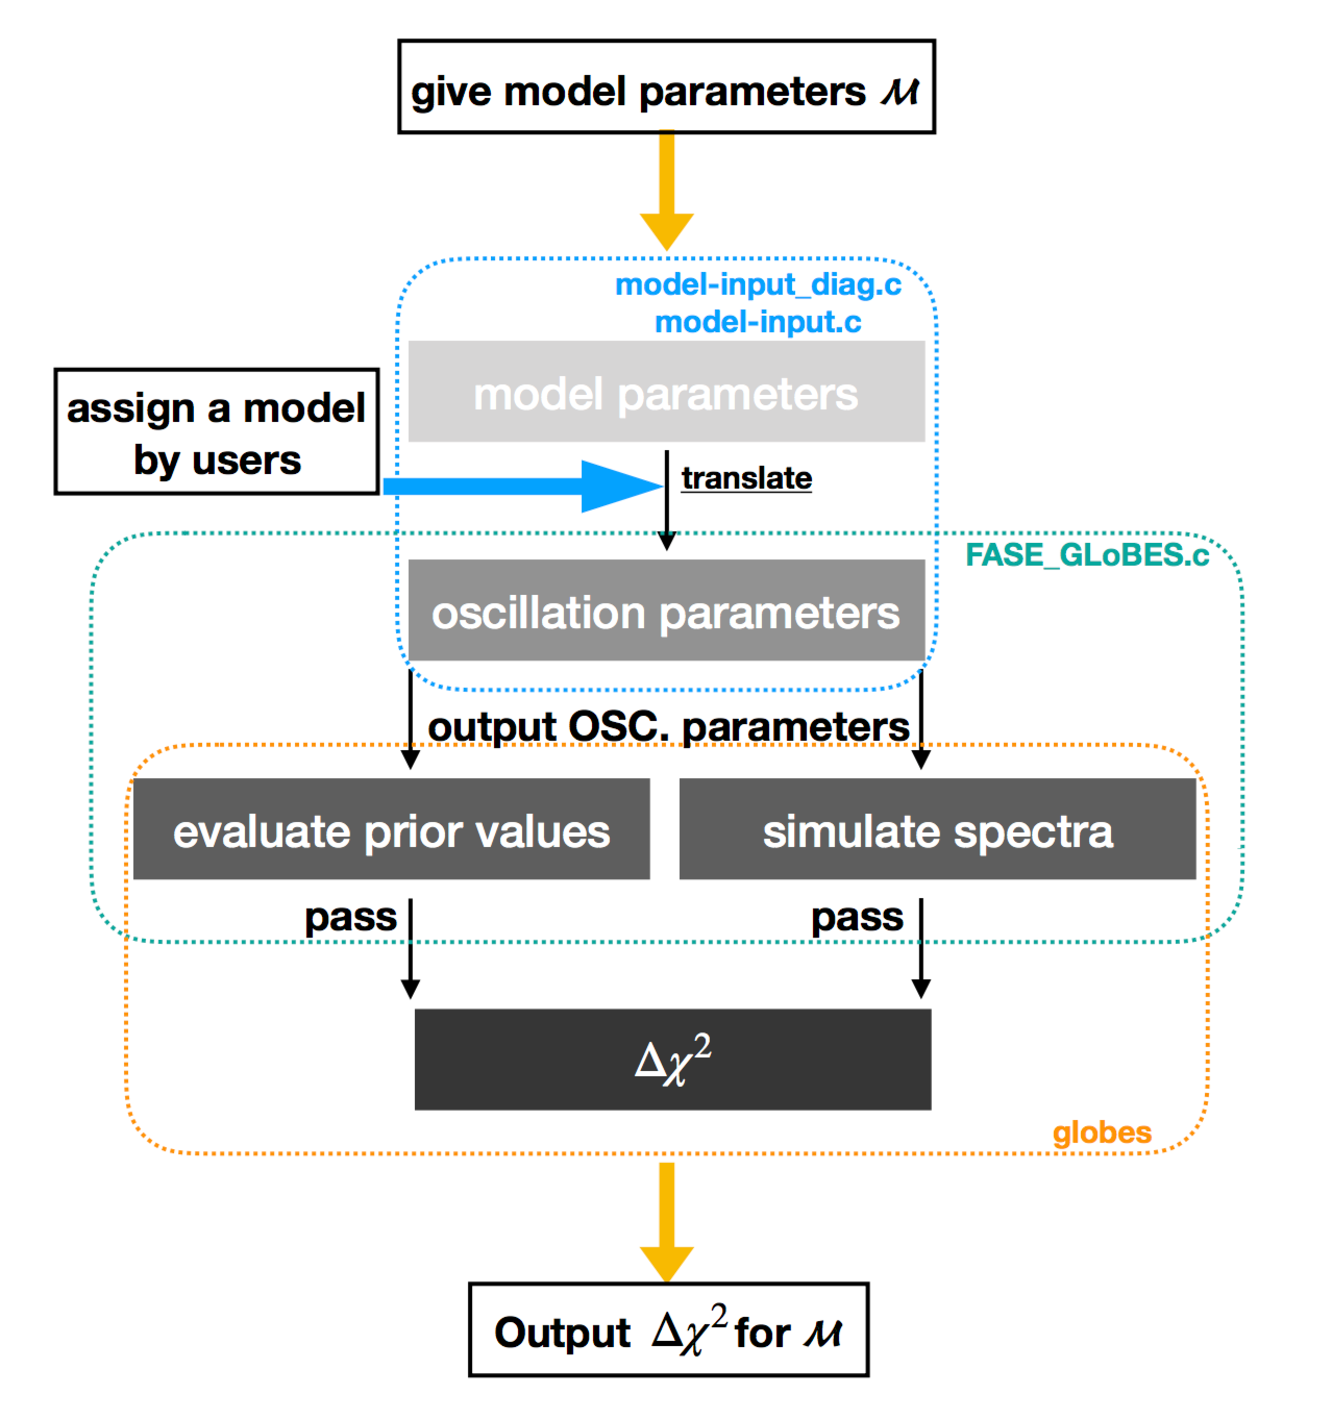
\includegraphics[width=4.5in]{Figs/FASE-chart_1_v1.pdf}
\caption{A scheme to correlate the model parameters with standard neutrino oscillation parameters. The error propagation is implemented in the simulation code up to the spectra analysis.}%
\label{fig:FASE}
\end{figure}


The concept of \textbf{FaSE-GLoBES} is shown in Fig.~\ref{fig:FASE}, in which three parts are shown: 1.~\textbf{the parameter translation} (the blue box), 2.~\textbf{giving oscillation-parameter values} (the green box), and 3.~\textbf{the $\chi^2$-value calculation} (the orange box). 
The idea behind this flow chart Fig.~\ref{fig:FASE} is that given a set of value for model parameter, the corresponding values for oscillation parameters are obtained by a translation, which is assigned by the user in \textbf{model-input.c}. And then, through \textbf{FASE\_GLoBES.c} these oscillation-parameter values are passed in to \textbf{GLoBES} library to simulate the event spectrum for evaluating the $\chi^2$ value. 


API functions in \textbf{FaSE} are listed:
\begin{enumerate}
\item \texttt{MODEL\_init($N_{para}$)},
\item  \texttt{FASE\_glb\_probability\_matrix},
\item  \texttt{FASE\_glb\_set\_oscillation\_parameters},
\item  \texttt{FASE\_glb\_get\_oscillation\_parameters},
\item \texttt{FASE\_prior\_OSC},
\item \texttt{FASE\_prior\_model}.
\end{enumerate}
The first one is to initialise \textbf{FaSE} with the number of input parameters $N_{para}$. The next three functions need to be included to replace the default \textbf{GLoBES} probability engine by the one that can read the output from \textbf{model-input.c}, as follows.\vspace{0.2cm}\\
\texttt{    glbRegisterProbabilityEngine(6,\\
                                 \&FASE\_glb\_probability\_matrix,\\
                                 \&FASE\_glb\_set\_oscillation\_parameters,\\
                                 \&FASE\_glb\_get\_oscillation\_parameters,\\
                                 NULL); }\vspace{0.2cm}\\ 
This probability engine can work with oscillation or model parameters. It can be set by the user with the parameter \texttt{PARA}. If \texttt{PARA=STAN} (\texttt{PARA=MODEL}) the probability engine works with oscillation (model) parameters. The final two items on the API list are prior functions. Once the user gives the prior in oscillation (model) parameters, the user needs to call \texttt{FASE\_prior\_OSC} (\texttt{FASE\_prior\_model}) as follows.\vspace{0.2cm}\\
\texttt{glbRegisterPriorFunction(FASE\_prior\_OSC,NULL,NULL,NULL); }  \\
or\\
\texttt{glbRegisterPriorFunction(FASE\_prior\_model,NULL,NULL,NULL); } \vspace{0.2cm}\\
We note that except for setting the probability engine and the prior function, the other parts in the main code should follow with the GLoBES manual. 

In the following, we give more details about using \textbf{FASE-GLoBES}. In Sec.~\ref{sec:download}, we will give the instruction to download and install \textbf{GLoBES} and \textbf{FASE}. Then, in Sec.~\ref{sec:compile}, we will introduce how to compile and run the code. More complicated is setting the model, and the way to do this will be described in Sec.~\ref{sec:model_set}. Finally, we will discuss how to set up the prior in Sec.~\ref{sec:prior}.


\subsection{Download and Installation}\label{sec:download}
\textbf{download and install GLoBES and FASE-GLoBES}\\
{\color{red}[will fill in after the code ready on Github]}

\subsection{Compile and Run}\label{sec:compile}
As \textbf{FaSE} works based on \textbf{GLoBES}, the user should use the \textbf{GLoBES} \texttt{Makefile}, but include the binary file of \textbf{FaSE}. To do so, we include the script in the \texttt{Makefile},\vspace{0.2cm}\\
\texttt{\{makefile\_execution\}: my\_program.o  FASE\_GLoBES.o model-input\_diag.o\\
	gcc my\_program.o  FASE\_GLoBES.o model-input\_diag.o -o my\_executable  \$(LDFLAGS) \$(local\_LDFLAGS)}\\
or\\
\texttt{\{makefile\_execution\}: my\_program.o  FASE\_GLoBES.o model-input.o\\
	gcc my\_program.o  FASE\_GLoBES.o model-input.o -o my\_executable  \$(LDFLAGS) \$(local\_LDFLAGS)}\vspace{0.2cm}\\	
where \texttt{\{compile\_execusion\}} is the makefile commend for the program \texttt{my\_program.o} and the execution \texttt{my\_executable} is the output. After giving this script in the \textbf{GLoBES} \texttt{Makefile}, the user needs to makefile the program \texttt{my\_program} on the terminal.\vspace{0.2cm}\\
\texttt{makefile \{makefile\_execution\}}\vspace{0.2cm}\\
And, the user can execute the program by typing the following commend on the terminal.\vspace{0.2cm}\\ 
\texttt{./my\_executable}\vspace{0.2cm}\\

The user can also compile the program without the \textbf{GLoBES} \texttt{Makefile} with the following script.\vspace{0.2cm}\\
\texttt{gcc my\_program.o FASE\_GLoBES.o model-input\_diag.o -lglobes -LGLB\_DIR/lib/ -o my\_executable}\\
or\\
\texttt{gcc my\_program.o FASE\_GLoBES.o model-input.o -lglobes -LGLB\_DIR/lib/ -o my\_executable}\vspace{0.2cm}\\
And, the execution is also in the same way: \texttt{./my\_executable}.\\

Finally we need to initialize \textbf{FaSE} by giving $N_{para}$ which is the number of model parameters. To do so, we need to include the following script in the main code.\\
\texttt{    MODEL\_init($N_{para}$); }\vspace{0.2cm}\\ 

\subsection{Model setting}\label{sec:model_set}

The function \texttt{MtoS} can do the translator from model parameters $\vec{\theta}_{Model}$ to oscillation parameters $\vec{\theta}_{OSC}$. After the user gives the array $\vec{\theta}_{Model}$ to the function \texttt{MtoS}, the output is the corresponding oscillation parameter $\vec{\theta}_{OSC}$, of which components are $\theta_{12}$, $\theta_{13}$, $\theta_{23}$, $\delta$, $\Delta m_{21}^2$, and $\Delta m_{31}^2$. For the first four components, values are given in the unit of \textbf{rad}, while the other two are in \textbf{eV$^2$}. These values will be passed in to \textbf{FaSE\_GLoBES} to simulate 
the experimental spectra and compute the prior value.


To do the translation from $\vec{\theta}_{Model}$ to $\vec{\theta}_{OSC}$, the user can assign the relation between the oscillation and model parameter sets, or define the mass matrix in model parameters, which will be diagonalised by the function \texttt{ModelTO} to obtain the corresponding oscillation-parameter values. 
%The relation between the oscillation and model parameter sets can be derived out by the user, 
In the way of directly giving the relation between oscillation and model parameter sets, the user needs to provide
\begin{equation}\label{eq:modelofOSC}
\vec{\theta}_{Model}=\vec{f}(\vec{\theta}_{OSC})
\end{equation}
 in the function \texttt{MtoS}.
%

The oscillation parameters can also be obtained in the way based on
\begin{equation}\label{eq:MM}
U^\dagger\mathcal{M}\mathcal{M}^\dagger U = \mathbf{M}^2,~\text{where}~\mathbf{M}^2_{\alpha\beta}=m_\alpha^2\delta_{\alpha\beta},
\end{equation}
where $\mathcal{M}$ ($\mathbf{M}$) is the neutrino mass matrix in the flavour (mass) state. The matrix $\mathcal{M}$ is given by user with model parameters $\vec{\theta}_{Model}$. The matrix $U$ is the neutrino mixing matrix, and can be used for getting mixing angles. The difference between any two diagonal elements of $\textbf{M}$ ($\textbf{M}_{ii}-\textbf{M}_{jj}=m_i^2-m_j^2$) is the mass-squared difference ($\Delta m_{ij}^2$). This diagnolisation Eq.~\ref{eq:MM} can be done with the function \texttt{ModelTO}, which needs to be called in \texttt{MtoS} and outputs directly the vector $\vec{\theta}_{OSC}$.

\subsection{Prior setting}\label{sec:prior}
Given a set of values for model parameters, \textbf{FASE\_GLoBES.c} will obtain the corresponding oscillation-parameter values from \textbf{model-input.c}, and will pass these values to simulate event spectra and to compute the prior value. Two gaussian prior functions are provided in \textbf{FaSE} -- \texttt{FASE\_prior\_OSC} and \texttt{FASE\_prior\_model}. These two functions are for different purposes. If the user give the prior in oscillation (model) parameters, the user should register \texttt{FASE\_prior\_OSC} (\texttt{FASE\_prior\_model}) with the \textbf{GLoBES} function \texttt{glbRegisterPriorFunction}, as we introduced in the beginning of this section. The user also needs to assign the parameter \texttt{PARA=STAN} (\texttt{PARA=Model}), when the user prefers to give the prior in oscillation (model) parameters. The Gaussian prior is 
\begin{equation}\label{eq:prior}
\chi^2_{prior}=\sum_{i} \frac{(\theta_i-\theta^c_i)^2}{\sigma_i^2},
\end{equation}
 where $\theta_i$ is one of parameters constrained by prior, $\theta^c_i$ ($\sigma_i$) is the central value (Gaussian width) of the prior for $\theta_i$. We note that $\theta_i$ can be either model ($\vec{\theta}_{Model}$) or oscillation parameters ($\vec{\theta}_{OSC}$).
%
The values of $\theta^c_i$ and $\sigma_i$ need to be given by the user through three arrays: \texttt{Central\_prior}, \texttt{UPPER\_prior}, and \texttt{LOWER\_prior}, in which there are six components. To treat asymmetry of width for upper ($\theta_i>\theta_i^c$) and lower ($\theta_i<\theta_i^c$) Gaussian widths, we give values in two arrays \texttt{UPPER\_prior}, and \texttt{LOWER\_prior}, respectively. If the user gives the prior in model parameters, the order of each component follows with the setup of input of the probability engine. While the user gives the prior in oscillation parameters, the six components in order are $\theta_{12}$, $\theta_{13}$, $\theta_{23}$, $\delta$, $\Delta m_{21}^2$, and  $\Delta m_{31}^2$. The first four parameter are in \textbf{rad}, and the final two are in \textbf{eV$^2$}.

Finally, some restrictions are imposed by the studied flavour symmetry model. We set up these restrictions in the function \texttt{model\_restriction} in \texttt{model-input.c}. In the function \texttt{model\_restriction}, the user needs to \textit{return $1$} once the restriction is broken. For example, if the normal ordering is imposed, we give ``\texttt{ if (DMS31<0) \{ return 1;\} } '' in \texttt{model\_restriction}, where \texttt{DMS31} is the variable for $\Delta m_{31}^2$. Then, when the restriction is broken, \texttt{model\_restriction} returns the value $1$ to the prior function \texttt{FASE\_prior\_OSC} or \texttt{FASE\_prior\_model}. Therefore, if there is no any restrictions, we simply \textit{return $0$} in \texttt{model\_restriction} as follows.\vspace{0.2cm}\\
\texttt{double model\_restriction(double model [])\{ return 0;\} }\vspace{0.2cm}\\

%In the following, the prior function will give $10^6$ for the $\chi^2$ value, and it will be selected out when the user studies the statistically reasonable region in the parameter space.  


\section{Examples}
\subsection{Setup for a model}
We now take the tri-direct littlest seesaw (TDLS)~\cite{King:2013iva,King:2015dvf,King:2016yvg} as an example. In this model, the atmospheric and solar flavon vacuum alignments are $\langle\phi_{\text{atm}}\rangle\propto\left(1, \omega^2, \omega\right)^T$ and $\langle\phi_{\text{sol}}\rangle\propto\left(1, x, x\right)^T$,
where  stands for a cube root of unity and the parameter $x$ is real because of the imposed CP symmetry. Under this model, the light left-handed Majorana neutrino mass matrix is given by
\begin{equation}
\label{eq:mnu}  m_{\nu}=m_{a}\begin{pmatrix}
 1 &~ \omega  &~ \omega ^2 \\
 \omega  &~ \omega ^2 &~ 1 \\
 \omega ^2 &~ 1 &~ \omega  \\
\end{pmatrix}+e^{i\eta}m_{s}
\begin{pmatrix}
 1 &~  x &~  x \\
 x &~ x^2 &~ x^2 \\
 x &~ x^2 &~ x^2 \\
\end{pmatrix}\,,
\end{equation}
where $x$, $\eta$, $m_a$, and the ratio $r\equiv m_s/m_a$ are four parameters and will be constrained by experimental data. We note that from Eq.~(\ref{eq:mnu}), $m_1=0$ and the normal mass ordering are imposed, and will need to be imposed in \textbf{FaSE-GLoBES}. Therefore, the restrictions in this model are $m_a>0$ and $r>0$.

\begin{table}[h!]
\caption{\label{tab:TD_parameters}A summary of the relation between oscillation parameters and TDLS model parameters~\cite{Ding:2018fyz}. Two requirements are imposed by TDLS: the smallest mass state $m_1=0$ and the normal mass ordering. The sign of $\sin\delta$ depends on the sign of $x\cos\psi$: ``$+$'' (``$-$'') is for $x\cos\psi>0$ ($<0$).}
\begin{tabular}{l|l}
\hline\hline
model parameters                                 & $x$, $\eta$, $r$, $m_a$                                                                                                                                                                         \\\hline
\multirow{6}{*}{combinations of model parameters} & $y=\frac{5x^2+2x+2}{2\left(x^2+x+1\right)}(m_{a}+e^{i \eta } m_{s})$,                                                                                                                            \\
                                                 & $z=-\frac{\sqrt{5x^2+2x+2}}{2\left(x^2+x+1\right)}\left[ (x+2)m_{a}-x(2x+1)e^{i \eta }m_{s}\right]$,                                                                                             \\
                                                 & $w=\frac{1}{2(x^2+x+1)}\left[(x+2)^2m_{a}+x^2\left(2x+1\right)^2e^{i \eta } m_{s}\right]$,                                                                                                       \\
                                                 & $\sin\psi=\frac{\Im\left(y^{*}z+wz^{*}\right)}{|y^{*}z+wz^{*}|},\quad \cos\psi=\frac{\Re\left(y^{*}z+wz^{*}\right)}{|y^{*}z+wz^{*}|}$.                                                           \\
                                                 & \begin{tabular}[c]{@{}l@{}}$\sin2\theta=\frac{2|y^{*}z+wz^{*}|} {\sqrt{(|w|^2-|y|^2)^2+4|y^{*}z+wz^{*}|^2}},$\end{tabular}                                                                     \\
                                                 & $\cos2\theta=\frac{|w|^2-|y|^2}{\sqrt{(|w|^2-|y|^2)^2+4|y^{*}z+wz^{*}|^2}}$.                                                                                                                     \\\hline
\multirow{7}{*}{oscillation parameters}          & $\Delta m_{21}^2=m^2_2=\frac{1}{2}\left[\left|y\right|^2+\left|w\right|^2+2\left|z\right|^2-\frac{\left|w\right|^2-\left|y\right|^2}{\cos\theta}\right]$,                                        \\
                                                 & $\Delta m_{31}^2=m^2_3=\frac{1}{2}\left[\left|y\right|^2+\left|w\right|^2+2\left|z\right|^2+\frac{\left|w\right|^2-\left|y\right|^2}{\cos\theta}\right]$,                                        \\
                                                 & $\sin^2\theta_{12}=1-\frac{3x^2 }{3x^2+2\left(x^2+x+1\right) \cos^2\theta }$,                                                                                                                  \\
                                                                                                  & $\sin^2\theta_{13}=\frac{2\left(x^2+x+1\right)\sin^2\theta}{5x^2+2x+2}$,                                                                                                                       \\
                                                 & $\sin^2\theta_{23}=\frac{1}{2}+\frac{x\sqrt{3\left(5x^2+2x+2\right)}\sin2\theta\sin\psi }{2\left[3x^2+2\left(x^2+x+1\right) \cos^ 2 \theta\right]}$,                                          \\
                                                 & $\cos\delta=\frac{ \cot 2 \theta_{23} \left[3x^2-\left(4x^2+ x+1\right)\cos^2\theta_{13}\right]}{\sqrt{3} \left|x\right| \sin \theta_{13} \sqrt{\left(5x^2+2x+2\right)\cos^2\theta_{13}-3x^2}}$, \\
                                                 & $\sin\delta= \pm\csc 2 \theta_{23} \sqrt{1+\frac{\left(x^2+x+1\right)^2 \cot ^2\theta_{13} \cos ^22 \theta_{23}}{3x^2 \left[3x^2 \tan ^2\theta_{13}-2 \left(x^2+x+1\right)\right]}}$.   \\\hline \hline       
\end{tabular}
\end{table}




\texttt{int MtoS(double OSC\_PARAMS[6],~double M\_para[])}\\
\texttt{\{}
\\        
   \texttt{double x=M\_para[0];}\\
    \texttt{double eta=M\_para[1];}\\
    \texttt{double r=M\_para[2];}\\
    \texttt{double ma=M\_para[3];}\\
    \texttt{double ms=ma*r;}\\
    
    \texttt{double complex Mass\_Matrix[] = \{ma+ms*(cos(eta) + I*sin(eta)), ma*(cos(6.6666e-1*M\_PI) + I*sin(6.6666e-1*M\_PI))+x*ms*(cos(eta) + I*sin(eta)), ma*(cos(6.6666e-1*M\_PI) + I*sin(6.6666e-1*M\_PI))*(cos(6.6666e-1*M\_PI) + I*sin(6.6666e-1*M\_PI))+x*ms*(cos(eta) + I*sin(eta)), ma*(cos(6.6666e-1*M\_PI) + I*sin(6.6666e-1*M\_PI))+x*ms*(cos(eta) + I*sin(eta)), ma*(cos(6.6666e-1*M\_PI) + I*sin(6.6666e-1*M\_PI))*(cos(6.6666e-1*M\_PI) + I*sin(6.6666e-1*M\_PI))+x*x*ms*(cos(eta) + I*sin(eta)), ma+x*x*ms*(cos(eta) + I*sin(eta)), ma*(cos(6.6666e-1*M\_PI) + I*sin(6.6666e-1*M\_PI))*(cos(6.6666e-1*M\_PI) + I*sin(6.6666e-1*M\_PI))+x*ms*(cos(eta) + I*sin(eta)), ma+x*x*ms*(cos(eta) + I*sin(eta)), ma*(cos(6.6666e-1*M\_PI) + I*sin(6.6666e-1*M\_PI))+x*x*ms*(cos(eta) + I*sin(eta))\};}\\
    
    \texttt{STAN\_OSC(Mass\_Matrix,OSC\_PARAMS);}\\
    
    \texttt{return 0;}\\
\texttt{\} }






\texttt{double MtoS(double osc\_para[6], double M\_para[])}\\
\texttt{\{}\\
    \texttt{/*example: tri-direct*/}\\
\\    
    \texttt{double x=M\_para[0];}\\
    \texttt{double eta=M\_para[1];}\\
    \texttt{double r=M\_para[2];}\\
    \texttt{double ma=M\_para[3];}\\
\\  
    \texttt{osc\_para[0]=TDth12(x,eta,r, ma);}\\
    \texttt{osc\_para[1]=TDth13(x,eta,r, ma);}\\
    \texttt{osc\_para[2]=TDth23(x,eta,r, ma);}\\
    \texttt{osc\_para[3]=TDdCP(x,eta,r, ma);}\\
    \texttt{osc\_para[4]=TDdm21(x,eta,r, ma);}\\
    \texttt{osc\_para[5]=TDdm31(x,eta,r, ma);}\\
\\    
    \texttt{return 0;}\\
\texttt{\}}\\

The functions \texttt{TDth12}, \texttt{TDth13}, \texttt{TDth23}, \texttt{TDdCP}, \texttt{TDdm21}, and \texttt{TDdm31} are included for obtaining the value of $\theta_{12}$, $\theta_{13}$, $\theta_{23}$, $\delta$, $\Delta m_{21}^2$, and $\Delta m_{31}^2$ according to Table~\ref{tab:TD_parameters}, respectively. 

The restrictions $m_a>0$ and $r>0$ need to be setup in \texttt{model\_restriction} as follows.\vspace{0.2cm}\\
\texttt{double model\_restriction(double model [])}\\
\texttt{\{}\\
\texttt{    double x=model[0];}\\
\texttt{    double eta=model[1];}\\
\texttt{    double r=model[2];}\\
\texttt{    double ma=model[3];}\\
    \\
\texttt{    if(ma<0) \{return 1;\}}\\
\texttt{    if(r<0) \{return 1;\}}\\
\\ 
\texttt{    return 0;}\\
\}\vspace{0.2cm}\\

\subsection{Initialise the code}
In the beginning of main code, we need to initialise GLoBES and FASE, and to include the AEDL file for the MuOn-decay MEdium baseline NeuTrino beam experiment (MOMENT)~\cite{Cao:2014bea} as follows.\vspace{0.2cm}\\ 
\texttt{glbInit(argv[0]);}\\
\texttt{glbInitExperiment("expMOMENT\_FIX\_FLUX\_150KM\_addATM\_NC.glb",\&glb\_experiment\_list[0],}\\
\texttt{\&glb\_num\_of\_exps);}\\
\texttt{MODEL\_init(4);}\vspace{0.2cm}\\
Then we register the probability engine.\vspace{0.2cm}\\
\texttt{glb\_init\_probability\_engine();}\\
\texttt{glbRegisterProbabilityEngine(6,\\
                                 \&FASE\_glb\_probability\_matrix,\\
                                 \&FASE\_glb\_set\_oscillation\_parameters,\\
                                 \&FASE\_glb\_get\_oscillation\_parameters,\\
                                 NULL); }\vspace{0.2cm}\\                                 
In the following we define the model-parameter values, and set the true value in model parameters.\vspace{0.2cm}\\
\texttt{     float degree   = M\_PI/180;}\\
\texttt{     float x\_true,eta\_true,r\_true,ma\_true;}\\
\texttt{    x\_true=-3.65029; eta\_true=1.13067*M\_PI; r\_true=0.511325; ma\_true=3.71199e-3;}\\
%
\texttt{glb\_params true\_values = glbAllocParams();}\\
\texttt{glb\_params test\_values = glbAllocParams();}\\
\texttt{glb\_params input\_errors  = glbAllocParams();}\\
\texttt{glb\_params centers         = glbAllocParams();}\\
\texttt{glbDefineParams(true\_values,x\_true,eta\_true,r\_true,ma\_true,0,0);}\\
\texttt{    glbSetDensityParams(true\_values,1.0,GLB\_ALL);}\\
\texttt{glbCopyParams(true\_values,test\_values);}\\
\texttt{PARA=MODEL;\\
    glbSetOscillationParameters(true\_values);\\
    glbSetRates();}\vspace{0.2cm}\\
We then finally set up the projection. The projection \texttt{free} is to set all four parameters free to find the minimal value of $\chi^2$, which \texttt{project} is used for studying the constraint on $x$ and $\eta$.\vspace{0.2cm}\\  
\texttt{glb\_projection projection = glbAllocProjection();\\
    glb\_projection free = glbAllocProjection();  \\
     glbDefineProjection(free,GLB\_FREE,GLB\_FREE,GLB\_FREE,GLB\_FREE,GLB\_FIXED,GLB\_FIXED);\\
    glbSetDensityProjectionFlag(free, GLB\_FREE, GLB\_ALL);\\
glbDefineProjection(projection,GLB\_FIXED,GLB\_FIXED,GLB\_FREE,GLB\_FREE,GLB\_FIXED\\ ,GLB\_FIXED);\\    
glbSetDensityProjectionFlag(projection, GLB\_FREE, GLB\_ALL);\\
    }
    
\subsection{Prior setup} 

To set up the prior, we need to register the prior function. As mentioned, when we use the prior in oscillation and model parameters, we register \texttt{FASE\_prior\_OSC} and \texttt{FASE\_prior\_model}, respectively. Here we present an example setting up priors in oscillation parameters according to NUFIT4.0 Table~\ref{tab:nufit4.0}.

\begin{table}[!h]
\caption{The best fit and $3\sigma$ uncertainty, in the results of NuFit4.0 \cite{Esteban:2018azc}.}
\begin{tabular}{|c|c|c|c|c|c|c|}
\hline
Parameter & $\theta_{12}/^\circ$ & $\theta_{13}/^\circ$ & $\theta_{23}/^\circ$ & $\delta/^\circ$  & $\Delta m_{21}^2/10^{-5}\text{eV}^2$ & $\Delta m_{31}^2/10^{-3}\text{eV}^2$\\ \hline\hline
best fit & $33.82$ & $8.61$ & $49.6$ & $215$ & $7.39$ & $2.525$ \\\hline
$3\sigma$ Range & $31.61-36.27$ & $8.22-8.99$ & $40.3-52.4$ & $125-392$ & $6.79-8.01$ & $2.47-2.625$ \\\hline
\end{tabular}
\label{tab:nufit4.0}
\end{table}

We therefore register \texttt{FASE\_prior\_OSC} for the prior function as follows.\vspace{0.2cm}\\
\texttt{glbRegisterPriorFunction(FASE\_prior\_OSC,NULL,NULL,NULL); }  \vspace{0.2cm}\\
And, then we give the value for the central values, and upper and lower Gaussian widths as follows.\vspace{0.2cm}\\
\texttt{    UPPER\_prior[0]=36.27*degree;  LOWER\_prior[0]=31.61*degree;   Central\_prior[0]=33.82*degree;}\\
\texttt{    UPPER\_prior[1]=8.99*degree; LOWER\_prior[1]=8.22*degree;  Central\_prior[1]=8.61*degree;}\\
\texttt{    UPPER\_prior[2]=52.4*degree;  LOWER\_prior[2]=40.3*degree;   Central\_prior[2]=49.6*degree;}\\
\texttt{    UPPER\_prior[3]=392*degree;  LOWER\_prior[3]=125*degree;   Central\_prior[3]=215*degree;}\\
\texttt{    UPPER\_prior[4]=8.01e-5;     LOWER\_prior[4]=6.79e-5;      Central\_prior[4]=7.39e-5; }\\
\texttt{    UPPER\_prior[5]=2.625e-3;     LOWER\_prior[5]=2.427e-3;      Central\_prior[5]=2.525e-3;}\\
   \\ 
\texttt{int i;}\\
\texttt{    for (i=0;i<6;i++) \{UPPER\_prior[i]=fabs(UPPER\_prior[i]-Central\_prior[i])/3; }\\
\texttt{                       LOWER\_prior[i]=fabs(LOWER\_prior[i]-Central\_prior[i])/3;\} }\\
\texttt{for (i=0; i<6; i++) glbSetOscParams(centers,0,i);}\\
\texttt{glbSetDensityParams(centers,1.0,GLB\_ALL);}
\texttt{glbCopyParams(centers,input\_errors);}\\
\texttt{    glbSetCentralValues(centers);   glbSetInputErrors(input\_errors);}\vspace{0.2cm}\\
The parameter \texttt{degree} is defined as $\pi/180$.

\subsection{Constraint of model parameters}


\begin{figure}[!h]
 %\flushleft
 \centering
\hspace{15mm}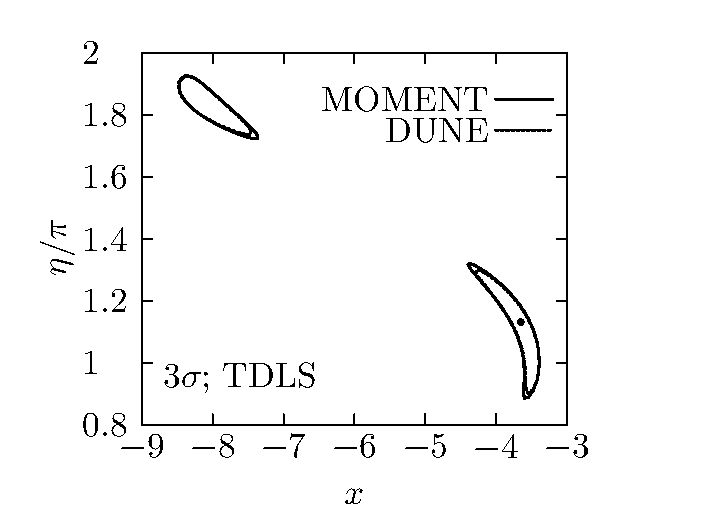
\includegraphics[width=0.5\textwidth]{figs/x_eta.pdf}
 \caption{\label{fig:x_eta}Precision measurements of any two model parameters in the framework of three neutrino oscillations taking uncertainties of the current global fit results, for MOMENT, at $1\sigma$ (gray), $2\sigma$ (orange), $3\sigma$ (black). True values for the model parameters are used $(x,~\eta,~r,~M_a)=(-3.65,~1.13\pi,~0.511,~3.71~\text{meV})$.}
\end{figure}


The user can use \textbf{FaSE-GLoBES} to study the constraint of model parameters. The expression of $\chi^2$ is used as the default \textbf{GLoBES} setting. In more detail, the $\chi^2$ function is constructed based on a log-likelihood ratio,
\begin{equation}\label{eq:chi-squared}
\chi^2(\vec{\theta},\xi_s,\xi_b)=2\sum_i\left(\eta_i(\vec{\theta},\xi_s,\xi_b)-n_i+n_i\ln\frac{n_i}{\eta_i(\vec{\theta},\xi_s,\xi_b)} \right)+p(\xi_s,\sigma_s)+p(\xi_b,\sigma_b)+\chi^2_{prior},
\end{equation}
where $i$ runs over the number of bins, $\eta_i(\vec{\theta},\xi_s,\xi_b)$ is the hypothesis event rate for bin i and $E_i$ is the central bin energy. The vector $\vec{\theta}$ consists of test model or oscillation parameters. The parameters $\xi_s$ and $\xi_b$ are introduced to account for the systematic uncertainty of normalisation for the signal (subscript $_s$) and background (subscript $_b$) components for the event rate, and are allowed to vary in the fit as nuisance parameters. For a given hypothesised set of parameters $\vec{\theta}$, the event rate for bin $i$ is calculated as\\
\begin{equation}
\eta_i(\vec{\theta},\xi_s,\xi_b)=(1+\xi_s)\times n_i+(1+\xi_b)\times b_i,
\end{equation}
where $n_i$ and $b_i$ are the expected number of signal and background events in bin $i$, respectively. The nuisance parameters are constrained by the Gaussian prior $p(\xi,\sigma)=\xi^2/\sigma^2$ with corresponding uncertainties $\sigma_s$ and $\sigma_b$ for the signal and background, respectively. Finally, $\chi^2_{prior}$ is a set of Gaussian priors for hypothesis, and is expressed as Eq.~\ref{eq:prior}. After doing all minimisations, the user obtain the $\chi^2$ value for a specific hypothesis $\vec{\theta}^{hyp}$, $\chi^2(\vec{\theta}^{hyp})$.

The user of \textbf{FaSE-GLoBES} is able to study how model parameters can be constrained by the simulated experiment. To do so, the user needs to define the true event spectrum $n_i$ with a set of model ($\vec{\theta}_{Model}^{true}$) or oscillation parameters ($\vec{\theta}_{OSC}^{true}$), \textit{i.e.}~set up $n_i(\vec{\theta}_{Model}^{true})$ or $n_i(\vec{\theta}_{OSC}^{true})$. The hypothesis $\vec{\theta}_{Model}^{hyp}$ predicts the tested event spectrum $\eta_i(\vec{\theta}_{Model}^{hyp},\xi_s,\xi_b)$. With the default setting for $\chi^2$ function Eq.~\ref{eq:prior}, from \textbf{FaSE-GLoBES} the user computes the statistical quantity,
\begin{equation}\label{eq:chi_model}
\chi^2(\vec{\theta}_{Model}^{hyp}),~~\text{with}~n_i(\vec{\theta}_{Model}^{true})~\text{or}~n_i(\vec{\theta}_{OSC}^{true}).
\end{equation}
%
We note that the minimum of $\chi^2$ in the whole parameter space ($\chi^2_{min.}$) may not be $0$. Therefore, to study the precision of model parameters, the user should use the value $\Delta\chi^2(\vec{\theta}_{Model}^{hyp})\equiv \chi^2(\vec{\theta}_{Model}^{hyp})-\chi^2_{min.}$, instead of $\chi^2$ itself. By varying different hypothesis $\vec{\theta}_{Model}^{hyp}$, the user can obtain the allowed region of model parameters with the statistical quantity $\Delta\chi^2(\vec{\theta}_{Model}^{hyp})$. 

We take TDLS as an example model, to see how the model parameter can be constrained by MOMENT experiment, assuming the true model values $x=-3.65$, $\eta=1.13\pi$, $r=0.511$, and $m_a=3.71$~meV. To get the constraint of $x$ and $\eta$, we need to comput the minimum of $\chi^2$ value as the following script in the main code.\vspace{0.2cm}\\
\texttt{
    glbSetProjection(free);\\
    float res0=glbChiNP(true\_values,NULL,GLB\_ALL);\\ } \vspace{0.2cm}\\
%
The \textbf{GLoBES} projector \texttt{free} allows all model parameters to vary, in order to find the value of \texttt{res0}, $\chi^2_{min}$.
Then, we set two loops varying different values of $x$ and $\eta$ in $\vec{\theta}^{hyp}_{Model}$ to get $\Delta \chi^2$ values for different hypotheses.\vspace{0.2cm}\\
%
\texttt{     float x,eta,r,ma,dx,deta;\\
     float lower\_x,upper\_x,lower\_eta,upper\_eta;\\
     FILE* File=fopen("data/constraint\_x\_eta.dat", "w");\\
    lower\_x=-9; upper\_x=-3; lower\_eta=0.8*M\_PI; upper\_eta=2*M\_PI;\\
    dx=(upper\_x-lower\_x)/100; deta=(upper\_eta-lower\_eta)/100;\\
        glbSetProjection(projection);\\
   for (x=lower\_x;x<=upper\_x;x=x+dx)\{ \\
    for (eta=lower\_eta;eta<=upper\_eta;eta=eta+deta)\{\\
     glbSetOscParams(test\_values,x,0); glbSetOscParams(test\_values,eta,1);\\
        float res=glbChiNP(test\_values,NULL,GLB\_ALL);\\
            fprintf(File,"\%f \%f  \%f $\backslash$n",x,eta/M\_PI,res-res0);\\
                     \} fprintf(File,"$\backslash$n");\}\\
}

The \textbf{GLoBES} projector \texttt{projection} fixes values of $x$ and $\eta$, but allows the other parameters to vary. The output (\texttt{data/contraint\_x\_eta.dat}) is a set of $\Delta \chi^2(\vec{\theta}^{hyp})$ (the third column) values with the changed $x$ (the first column), $\eta$ (the second column). We use these data, and obtain the predicted $1\sigma$, $2\sigma$, and $3\sigma$ constraints of $x$ and $\eta$ by MOMENT shown in Fig.~\ref{fig:x_eta}. The code for this example is provided as \textbf{x\_eta.c} in the \textbf{FaSE} distribution.
 
%\begin{figure}[!h]
% \flushleft
%\hspace{15mm}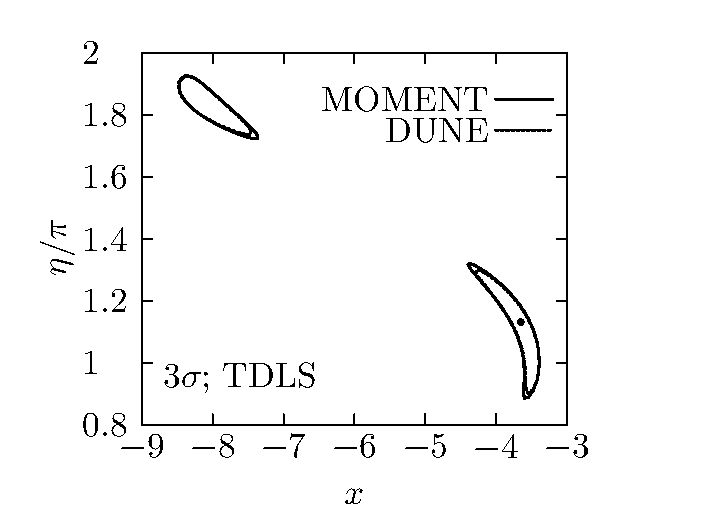
\includegraphics[width=0.32\textwidth]{figs/x_eta.pdf}$~~~~~~$\\
%\hspace{15mm} 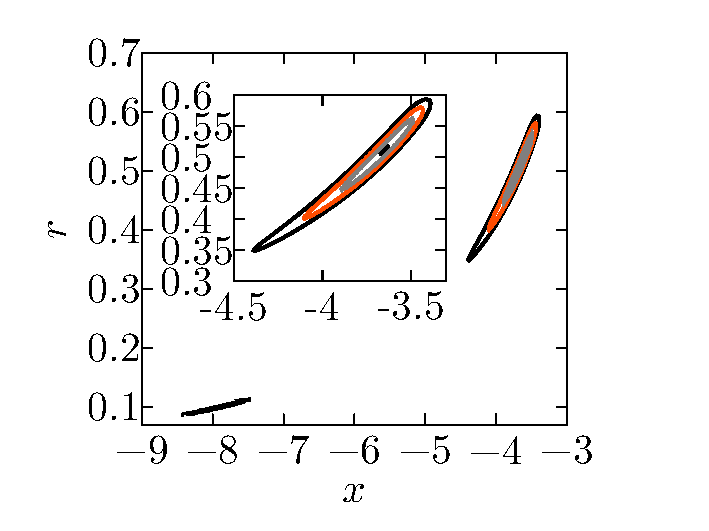
\includegraphics[width=0.32\textwidth]{figs/x_r.pdf}\hspace{-11mm}
% 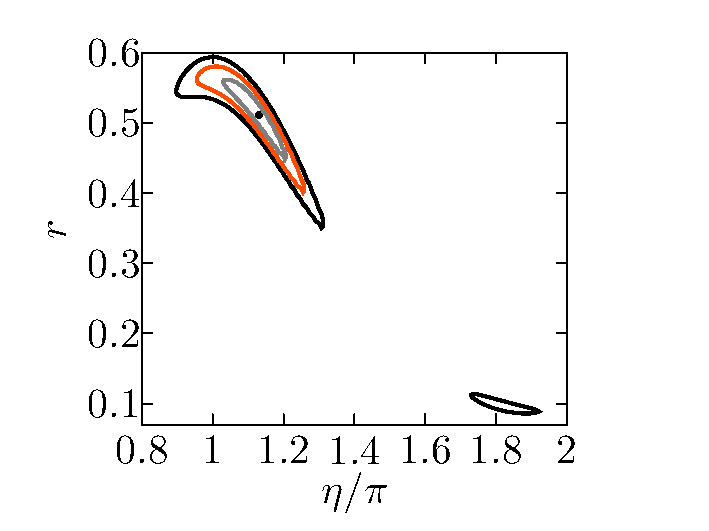
\includegraphics[width=0.32\textwidth]{figs/eta_r.pdf}$~~~~~~$\\
%\hspace{15mm} 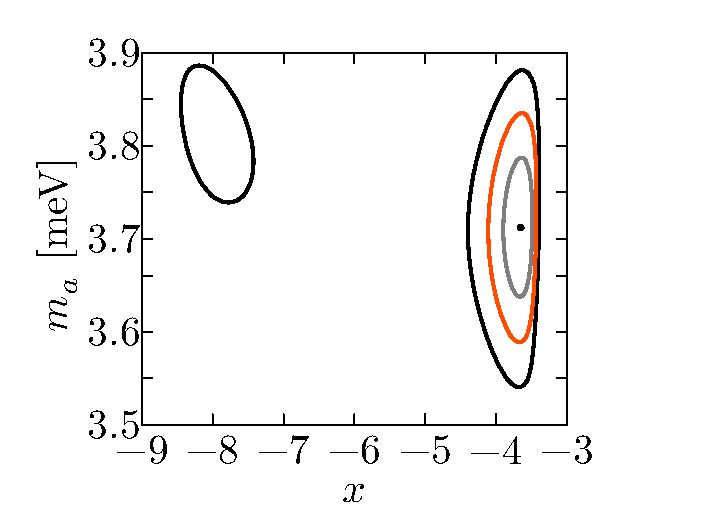
\includegraphics[width=0.32\textwidth]{figs/x_ma.pdf}\hspace{-11mm}
% 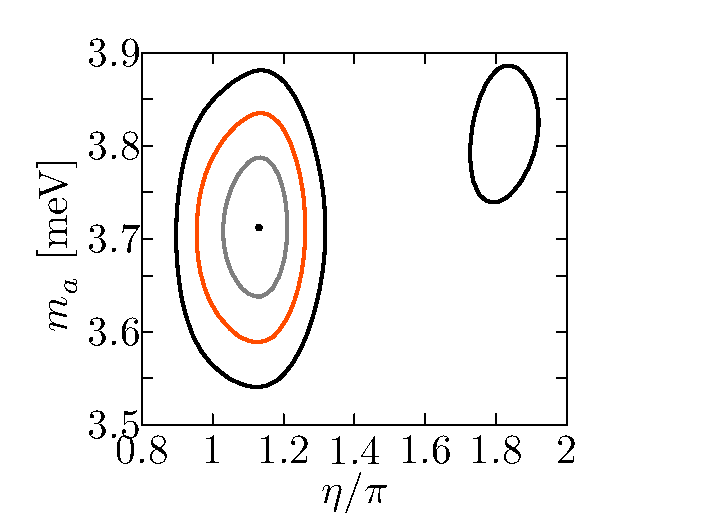
\includegraphics[width=0.32\textwidth]{figs/eta_ma.pdf}\hspace{-11mm}
% 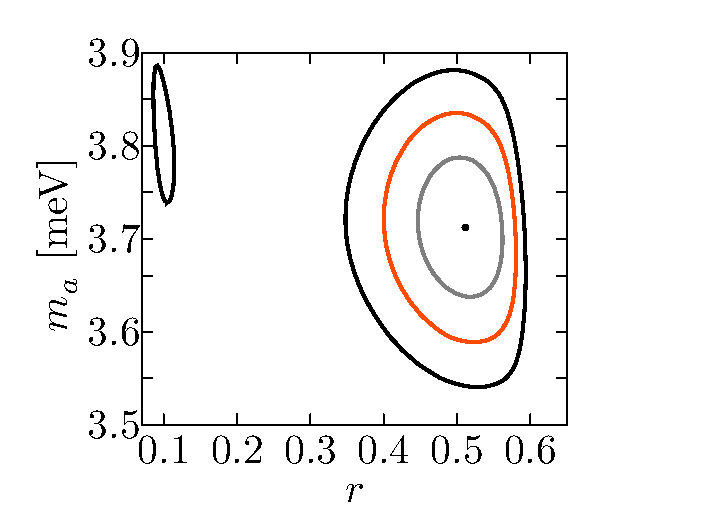
\includegraphics[width=0.32\textwidth]{figs/r_ma.pdf}
% \caption{\label{fig:model_2D}Precision measurements of any two model parameters at 3$\sigma$ confidence level in the framework of three neutrino oscillations taking uncertainties of the current global fit results, for MOMENT, at $1\sigma$ (gray), $2\sigma$ (orange), $3\sigma$ (black). True values for the model parameters are used $(x,~\eta,~r,~M_a)=(-3.65,~1.13\pi,~0.511,~3.71~\text{meV})$.}
%\end{figure}



%\texttt{
%glbFreeParams(true\_values);\\
%glbFreeParams(test\_values); \\
%glbFreeParams(input\_errors); \\
%glbFreeParams(centers);\\
%glbFreeProjection(free);\\
%glbFreeProjection(projection);\\
%}



\subsection{Model testing}

The user can also study how well a flavour symmetry model explains the computed data as predicting how the simulated experiment can exclude this model. In the other word, the user studies the minimum of $\chi^2$ for the flavour symmetry model $\vec{\theta}_{Model}$ as a hypothesis, assuming different true oscillation values, \textit{i.e.}~different $\vec{\theta}^{true}_{OSC}$. To do so, we compute the same statistical quantity Eq.~\ref{eq:chi_model}, while the true spectrum is varied with different true values $\vec{\theta}_{OSC}^{true}$. All model parameters are allowed to be varied with the user-defined prior.
%
Finally, the user needs to adopt Wilk's theorem \cite{Wilks:1938dza}. When comparing nested models, the $\Delta \chi^2$ test statistics is a random variable asymptotically distributed according to the $\chi^2$-distribution with the number of degrees of freedom, which is equal to the difference in the number of free model parameters \texttt{dof}. 


\begin{figure}[!h]
 \centering
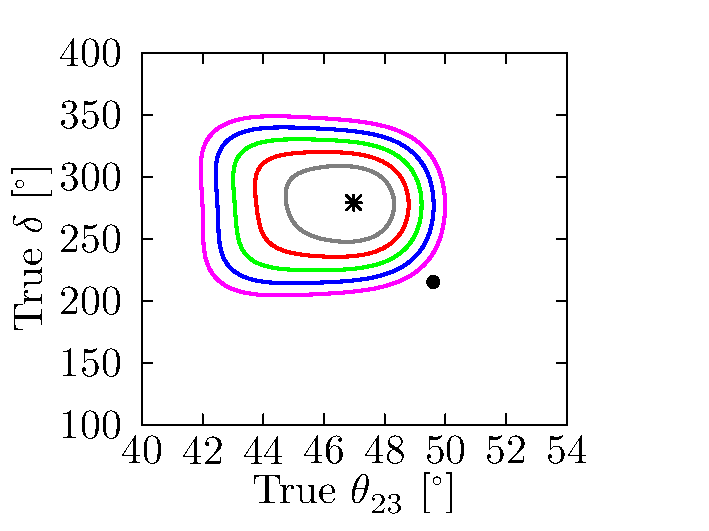
\includegraphics[width=0.5\textwidth]{figs/SR_th23_dCP.pdf}
\caption{\label{fig:th23_delta}The 2-D exclusion contour for tri-direct littlest seesaw model on the plane of two true standard parameters $\theta_{23}$ and $\delta$, from $1\sigma$ to $5\sigma$. The range for each parameter is taken according to the $3\sigma$ uncertainty in NuFit4.0 results. The black dot denotes the best fit of NuFit4.0 results ($(\theta_{12},~\theta_{13},~\theta_{23},~\delta,~\Delta m_{21}^2,~\Delta m_{31}^2)=(33.82^\circ,~8.61^\circ,~49.6^\circ,~215^\circ,~7.39\times10^{-5}~\text{eV}^2,~2.525\times10^{-3}~\text{eV}^2)$), while the star is the prediction by the tri-direct littlest seesaw model with NuFit4.0 results ($(\theta_{12},~\theta_{13},~\theta_{23},~\delta,~\Delta m_{21}^2,~\Delta m_{31}^2)\sim(36.25^\circ,~8.63^\circ,~47^\circ,~279^\circ,~7.39\times10^{-5}~\text{eV}^2,~2.525\times10^{-3}~\text{eV}^2)$).}
\end{figure}

%We can also study on excluding the model, assuming different true values for oscillation parameters. 
As an example, we present testing TDLS, assuming various true values of $\theta_{23}$ and $\delta$. The code for this example is provided as \textbf{th23\_delta.c}. in the \textbf{FaSE} distribution We change values of $\theta_{23}$ and $\delta$ of the true theory, and compute the minimal $\chi^2$ value for the tested model with all four model parameters, allowed to vary with priors. And, the studied statistics function is exactly Eq.~\ref{eq:chi-squared}, but the true event rate $n_i$ is predicted by a set of oscillation parameters, which will be varied in the code. And all four model parameter can be varied with the prior given by Eq.~\ref{eq:prior}. 
%
Except for $\theta_{23}$ and $\delta$, which are varied between $40^\circ<\theta_{23}<52^\circ$ and $125^\circ<\delta<392^\circ$, we fix the other oscillation parameters at $\theta_{12}=36.25^\circ$, $\theta_{13}=8.63^\circ$, $\Delta m_{21}^2=7.39\times 10^{-5}$~eV$^2$ and $2.525\times10^{-3}$~eV$^2$ predicted by the model $x=-3.65$, $\eta=1.13\pi$, $r=0.511$, and $m_a=3.71$~meV. 

The example code is presented as follows.\vspace{0.2cm}\\
\texttt{ \{ ...  initalize the code ...\}\\
\{ ...  register the probability engine ...\}    }\vspace{0.2cm}\\
\texttt{    
    float degree   = M\_PI/180;\\
    float x\_true,eta\_true,r\_true,ma\_true;\\
    x\_true=-3.65029; eta\_true=1.13067*M\_PI; r\_true=0.511325; ma\_true=3.71199e-3;\\
    double M\_para[4],OSC\_para[6];\\
    M\_para[0]=x\_true; M\_para[1]=eta\_true; M\_para[2]=r\_true; M\_para[3]=ma\_true;\\
    MtoS(OSC\_para, M\_para);\\
    double th12\_true=OSC\_para[0];\\
    double th13\_true=OSC\_para[1];\\
    double th23\_true=OSC\_para[2];\\
    double dCP\_true=OSC\_para[3];\\
    double DM21\_true=OSC\_para[4];\\
    double DM31\_true=OSC\_para[5];\\
    glb\_params true\_values = glbAllocParams();\\
    glb\_params test\_values = glbAllocParams();\\
    glb\_params input\_errors = glbAllocParams();\\
    glb\_params centers = glbAllocParams();\\
    \\
    glbDefineParams(test\_values,x\_true,eta\_true,r\_true,ma\_true,0,0);\\
    glbSetDensityParams(test\_values,1.0,GLB\_ALL);\\
    glbDefineParams(true\_values,th12\_true,th13\_true,th23\_true,dCP\_true,\\
    DM21\_true,DM31\_true);\\
    glbSetDensityParams(true\_values,1.0,GLB\_ALL); }\vspace{0.2cm}\\
\texttt{ \{ ...  set up for prior ...\}}\vspace{0.2cm}\\
\texttt{
    float th23,dCP,dth23,ddCP,lower\_th23,upper\_th23,lower\_dCP,upper\_dCP;\\
    FILE* File=fopen("data/ModelTest\_th23\_dCP\_test.dat", "w");\\
    lower\_th23=40; upper\_th23=52; lower\_dCP=125; upper\_dCP=392;\\
    dth23=(upper\_th23-lower\_th23)/100; ddCP=(upper\_dCP-lower\_dCP)/100;\\
    glbSetProjection(free);\\
    for (th23=lower\_th23;th23<=upper\_th23;th23=th23+dth23)\{\\
    for (dCP=lower\_dCP;dCP<=upper\_dCP;dCP=dCP+ddCP)\{\\
    glbSetOscParams(true\_values,th23*degree,GLB\_THETA\_23);\\
    glbSetOscParams(true\_values,dCP*degree,GLB\_DELTA\_CP);\\
    PARA=STAN; \\
    glbSetOscillationParameters(true\_values);\\
    glbSetRates();\\
    PARA=MODEL;\\ 
        float res=glbChiNP(test\_values,NULL,GLB\_ALL);\\
            fprintf(File,"\%f \%f \%f $\backslash$n",th23,dCP,\\
            gsl\_cdf\_chisq\_Qinv(gsl\_cdf\_chisq\_Q(fabs(res),dof),1));\\
         \} fprintf(File,"$\backslash$n");\\
    \}
}\vspace{0.2cm}\\
\texttt{ \{ ...  destroy the pointer ...\}}\vspace{0.2cm}\\
Finally, in the code we adopt Wilk's theorem \cite{Wilks:1938dza}. Here the number \texttt{dof} is $2$. And that is our output: \texttt{gsl\_cdf\_chisq\_Qinv(gsl\_cdf\_chisq\_Q(fabs(res),dof),1)}.

%\begin{figure}[!h]
 %\flushleft
%
%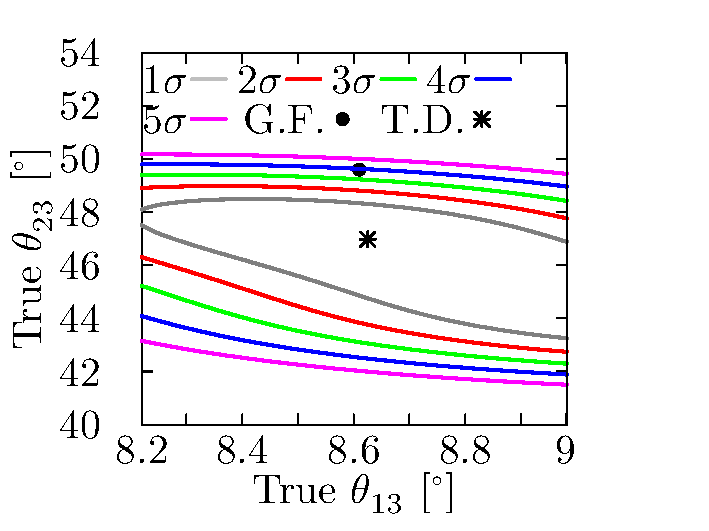
\includegraphics[width=0.32\textwidth]{figs/SR_th13_th23.pdf}$~~~~~~$\\
%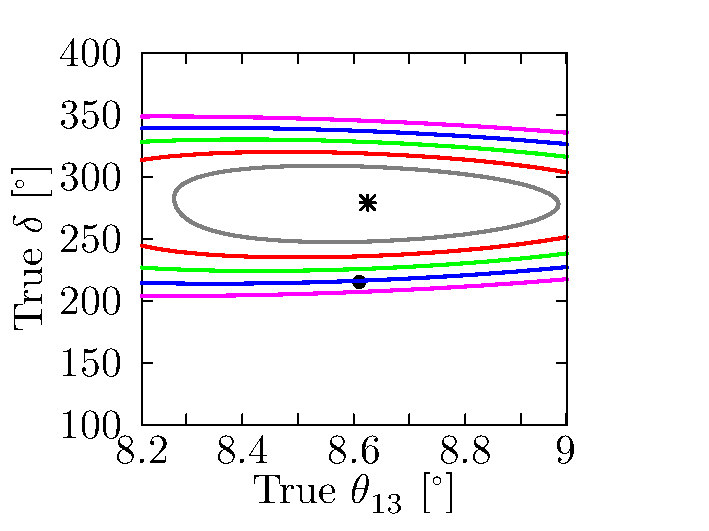
\includegraphics[width=0.32\textwidth]{figs/SR_th13_dCP.pdf}
%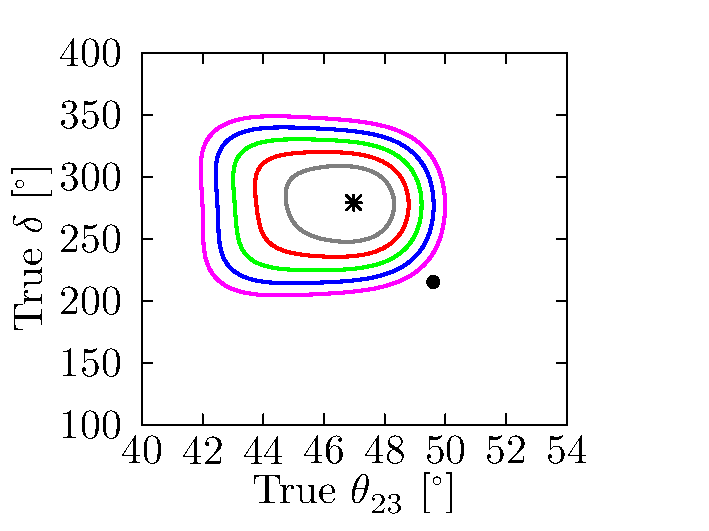
\includegraphics[width=0.32\textwidth]{figs/SR_th23_dCP.pdf}$~~~~~~$\\
%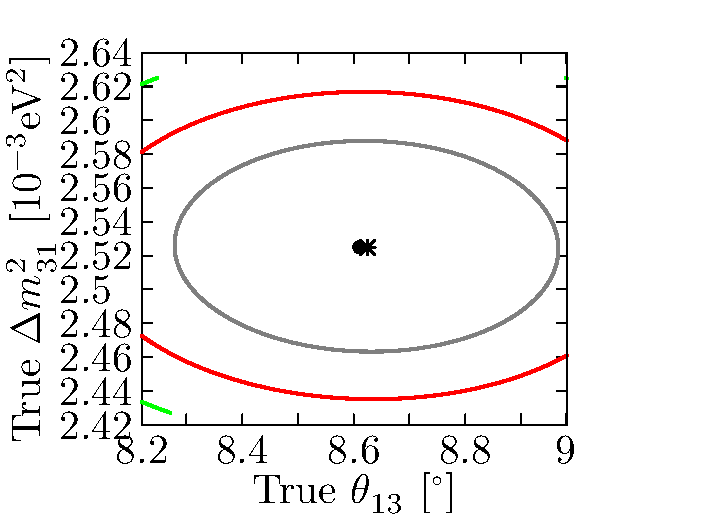
\includegraphics[width=0.32\textwidth]{figs/SR_th13_ldm.pdf}
%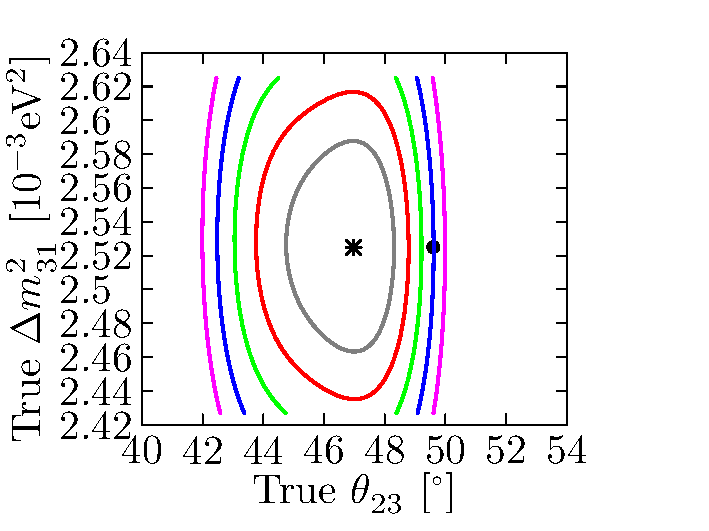
\includegraphics[width=0.32\textwidth]{figs/SR_th23_ldm.pdf}
%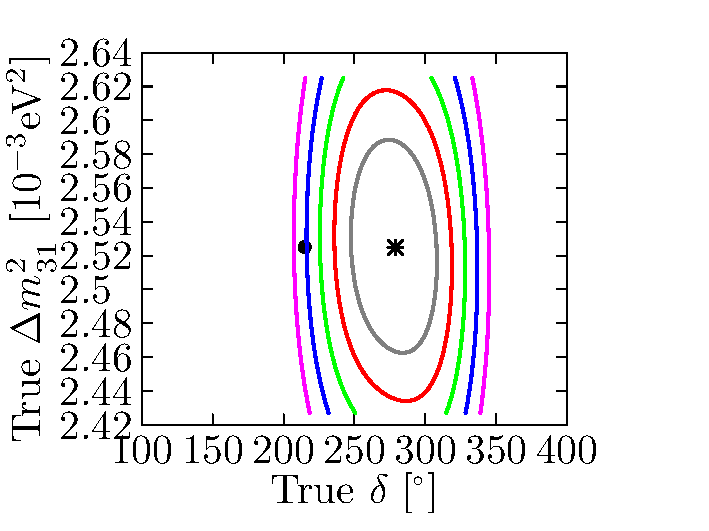
\includegraphics[width=0.32\textwidth]{figs/SR_dCP_ldm.pdf}
% \caption{\label{fig:SR_2D}The 2-D exclusion contour for tri-direct littlest seesaw model on the plane of any two true standard parameters, from $1\sigma$ to $5\sigma$. The range for each parameter is taken according to the $3\sigma$ uncertainty in NuFit4.0 results. The black dot denotes the best fit of NuFit4.0 results ($(\theta_{12},~\theta_{13},~\theta_{23},~\delta,~\Delta m_{21}^2,~\Delta m_{31}^2)=(33.82^\circ,~8.61^\circ,~49.6^\circ,~215^\circ,~7.39\times10^{-5}~\text{eV}^2,~2.525\times10^{-3}~\text{eV}^2)$), while the star is the prediction by the tri-direct littlest seesaw model with NuFit4.0 results ($(\theta_{12},~\theta_{13},~\theta_{23},~\delta,~\Delta m_{21}^2,~\Delta m_{31}^2)\sim(36.25^\circ,~8.63^\circ,~47^\circ,~279^\circ,~7.39\times10^{-5}~\text{eV}^2,~2.525\times10^{-3}~\text{eV}^2)$).}
%\end{figure}



The output \texttt{data/ModelTest\_th23\_dCP\_test.dat} contains true values of $\theta_{23}$ (the first column) and $\delta$ (the second column) with $\chi^2_{min}$ for TDLS (the third column). With these data, we then have the results shown in Fig.~\ref{fig:th23_delta}.

\section{Summary and conclusions}

We have presented \textbf{FaSE}, which is a supplemental simulation tool for \textbf{GLoBES} to study the flavour symmetry with neutrino oscillation experiments. \textbf{FaSE} provides \texttt{c}-codes: \textbf{model-input.c} and \textbf{FASE\_GLoBES.c}. Shown in Fig.~\ref{fig:FASE}, \textbf{FASE\_GLoBES}, which calls functions in \textbf{model-input.c}, plays a role as a bridge between \textbf{FaSE} and \textbf{GLoBES} to simulate the expected spectra and compute the prior value. It can be left to be untouched by users. However, all inputs of the user needs to be given in the code \textbf{model-input.c}. Given a set of model parameters $\vec{M}$, with \textbf{GLoBES}, the output can be the $\chi^2$ value for the hypothesis $\vec{M}$. {\color{red}\texttt{Makefile} is easy to include these two binary files (\textbf{model-input} and \textbf{FASE\_GLoBES}) in the \texttt{makefile} script for \textbf{GLoBES}. }

We also present two examples for \textbf{FaSE-GLoBES} with the flavour symmetry model -- tri-direct littlest seesaw (TDLS) -- and the future neutrino oscillaiton experiment -- MOMENT. We show the model can be assign in two ways: the relation between model and oscillation parameters or the form of mass matrix in model parameters. The input of the oscillation probability and prior value can be in model or oscillation parameters. We further demonstrate how to use \textbf{FaSE-GLoBES} to obtain the constraint of any two of model parameters, and to study the ability to TDLS by MOMENT experiment. 

Finally, \textbf{GLoBES} is a popular and powerful simulation tool to analysis the neutrino oscillation experiments in a simple language (AEDL), without losing too much detail. Considering the success of the flavour symmetry theory to explain the neutrino oscillations, \textbf{FaSE-GLoBES} should benefit model builders of leptonic flavour symmetry and phenomenologists for neutrino oscillation physics. We leave the flexibility for the user, and some other improvements and extensions might be done in the future.
 

% BIBLIOGRAPHY
% use BIBTEX if you want
\bibliographystyle{JHEP}
%\bibliographystyle{plain}
\bibliography{FAS-GLoBES.bib}
\end{document}
